\subsection{Stochastic Games}
We consider a graph-based game formalism between two players. A
(2.5-player) \emph{stochastic game} (SG) is a tuple $\sg = \langle S,
\iota, \Act, P \rangle$.  The finite set of \emph{states} $S = S_\pOne \cup
S_\pTwo$ is partitioned into a set $S_\pOne$ of (controlled)
$\pOne$-states and a set $S_\pTwo$ of (uncontrolled)
$\pTwo$-states. $\iota \in S_\pOne$ is the \emph{initial state}, $\Act$ is a
finite set of \emph{actions}, and $P\colon S \times \Act \rightarrow
\Distr(S)$ is the \emph{transition function}. For simplicity of
exposition, we assume w.l.o.g. that controlled and uncontrolled
states alternate. Thus, $P$ is defined by two partial transition functions:
$P_\pOne\colon S_\pOne \times \Act \rightarrow \Distr(S_\pTwo)$,
$P_\pTwo\colon S_\pTwo \times \Act \rightarrow \Distr(S_\pOne)$. We
identify the available actions\footnote{We explicitly allow to model
unavailable actions, e.g., we can model that a door can only opened
when close enough to the door.} as $\EnAct(s) \eqdef \{ \act \mid
P(s,\act) \neq \bot \}$. States without available actions, i.e.,
states with $\EnAct(s) = \emptyset$ are called \emph{terminal states}.
The \emph{successor
states} of a state $s$ and an (enabled) action $\act$ is the set of
states that are reached from $s$ within one step with a positive
transition probability, i.e., $\Succ(s,\act) \eqdef \{ s' \mid
P(s,\act)(s')>0 \}$, and $\Succ(s) \eqdef\bigcup_{\act \in \EnAct(s)}
\Succ(s,\act)$.


\begin{figure}
\centering
\begin{tikzpicture}
	\node[sstate,initial,initial text=] (s0) {$s_0$};
	\node[astate,right=of s0] (s1) {$s_1$};
	\node[astate,below=of s0] (s2) {$s_2$};
	
	\node[sstate,below=of s1] (s3) {$s_3$};
	
	\node[tstate,right=1.4cm of s1] (target) {$\target$};
	\node[tstate,right=1.4cm of s3] (sink) {$\sink$};
	
	\node[actnode,right=4mm of s1] (a1) {};
	\node[actnode,right=4mm of s3] (a2a) {};
	
	
	\draw[->] (s0) -- node[actnode] {} 
	                  node[near start,auto,elab] {$a$} (s1);
	\draw[->] (s0) -- node[actnode] {}
					  node[near start,elab,right] {$b$} (s2);
					  
	\draw[->] (s2) -- node[actnode] {}
					  node[near start,elab,above] {$a$} (s3);				  
					  
	\draw[->] (s1) -- node[actnode] {}
					  node[near start,elab] {$b$}  (s3);
	\draw[->] (s1) -- node[elab] {$a$} (a1);
	\draw[->] (a1) -- node[elab] {$\nicefrac{1}{3}$} (target);
	\draw[->] (a1) -- node[elab,near start,left] {$\nicefrac{2}{3}$} (sink);
	\draw[->] (a2a) -- node[elab,near start,xshift=0.1cm] {$\nicefrac{1}{3}$} (target);
	\draw[->] (a2a) -- node[elab,pos=0.6,above] {$\nicefrac{2}{3}$} (sink);
	\draw[->] (s3) -- node[elab] {$a$} (a2a);
	\draw[->] (s3) edge[bend right=30] node[actnode] {}
										node[near start,below] {$b$} (sink);
	
	
\end{tikzpicture}	
\caption{A running example. }
\label{fig:toysg}
\end{figure}
\begin{example}
  We introduce a six-state toy-example~(Fig.~\ref{fig:toysg}) to
  illustrate the formalisms. Terminal states are drawn with a rectangle,
  $\pOne$-states with a circle and $\pTwo$-states with a diamond. For
  every state $s$ and action $\act$, we draw transitions in the form
  of edges that connect all successors $s'$, and label them with the
  associated probabilities $P(s,\act)(s')$. For conciseness, we omit
  labelling probability $1$ transitions.
\end{example}
	

SGs capture a variety of models.  For example, if $|\EnAct(s)| = 1$ for all uncontrolled states $s \in S_\pTwo$, then $\sg$ is a
\emph{Markov decision process} (MDP).  If $|\EnAct(s)| = 1 $ for all $s \in S$, then $\sg$ is a \emph{Markov chain}. If
$P(s,\act)$ is a Dirac distribution for every $s \in S$ and $\act \in
\Act$, then $\sg$ is called \emph{deterministic} or a \emph{2-player
game}.

\subsection{Paths and Path Properties}
A finite \emph{path}, $\path$, of length $n$ is a sequence $s_0
\xrightarrow{\act_0} s_1 \xrightarrow{\act_1} s_2 \rightarrow \hdots
\rightarrow s_n$ in $\left( S \times \Act \right)^{n} \times S$ where
$P(s_i,\act_i)(s_{i+1}) > 0$ for each $i$.  We denote the length with
$|\path|$, and denote $s_n$, i.e., the last element of $\path$ with
$\last{\path}$. Further, note that $\pOne$ states are even
indexed and $\pTwo$ states are odd indexed as we assume alternation.
A path, $\path' = s'_0 \xrightarrow{\act'_0} \hdots$, is a
\emph{prefix} of $\path$, if for all $i \leq |\path'|$, $s_i = s'_i$
and for all $i < |\path'|$, $\act_i = \act'_i$.  The set of all finite
paths of length $n$ is denoted $\Paths[n]{\sg}$, and $\Paths{\sg} =
\bigcup_{n \in \NN} \Paths[n]{\sg}$. We omit $\sg$ whenever it is
irrelevant or clear from the context.
It is helpful to partition paths
based on their last state: $\POnePaths[]{} = \{ \path \in
 \Paths[]{} \mid \last{\path} \in S_\pOne \}$ and $\PTwoPaths[]{} =
\Paths[]{} \setminus \POnePaths[]{}$.



\begin{example}
  In Fig.~\ref{fig:toysg}, there are two paths that end in $s_3$, $s_0 \xrightarrow{a} s_1 \xrightarrow{b} s_3$ and $s_0 \xrightarrow{b} s_2 \xrightarrow{a} s_3$, both of length $1$. Both paths are in $\POnePaths[]{}$, as $s_3 \in S_\pOne$.
\end{example}
%\paragraph{Policies.} 
Whenever some state $s$ is reached, the corresponding player draws an action from $\EnAct(s)$. As standard, we capture this with the notion of a scheduler\footnote{Also known as \emph{strategy} or \emph{policy}.}.
A \emph{scheduler} is a tuple of \emph{player policies} $\sched = \langle \sched_\pOne, \sched_\pTwo \rangle$
with $\sched_{\player} \colon \PlayerPaths[]{} \rightarrow \Distr(\Act)$ such that $\supp(\sched_i(\path)) \subseteq \EnAct(\last{\path})$ for each $\path$, i.e., for every history, the policy sets a distribution over the enabled successor actions.
We will denote by $\sched_{\player}(\act~|~\path)$ the distribution of actions given the path, $\path$, induced by policy $\sched_{\player}$.
%We refer to $\sched_i$, $i \in \{ 1, 2 \}$ as a \emph{Player-i policy}. 
%We denote the $\pOne$-policy $\pOneSched$ and the $\pTwo$-policy $\pTwoSched$ with $\sched_\pOne$ and $\sched_\pTwo$, respectively.
To ease notation, we liberally use the notation $\sched \colon \Paths{} \rightarrow \Distr(\Act)$ where this function is given dependent on which player owns the last state.
 
%
%Applying a policy $\sched$ to an SG $\sg$ yields an \emph{induced Markov chain} $\induced{\sg}{\sched} = \langle S', \iota', P' \rangle$ with state space $S' = \Paths{\sg}$, initial state $\iota' = \iota$, and transition function $P'(\path,\path')$ defined by $P'(\path)(\path \cdot \act s') = \sched(\path)(\act) \cdot P(\last{\path},\act)(s')$ and $P'(\path,\path') = 0$ otherwise. For any upper bound on the length of the paths, the induced MC is finite. 


\begin{example}
  An example for a $\pOne$-policy $\pOneSched$ is given
  by,
  \begin{equation}
    \pOneSched(\alpha~|~\xi) =
    \begin{cases}
      1 & \text{if } \alpha \in \{ a,b \}, ~\xi = s_0\\
      \nicefrac{1}{2} & \text{if } \alpha = a,~\xi = s_0\xrightarrow{b}s_2 \xrightarrow{a} s_3\\
      1 & \text{if } \alpha = b,~\xi = s_0\xrightarrow{a}s_1\xrightarrow{b}s_3\\
    \end{cases}.
  \end{equation}
\end{example}


%\paragraph{Properties.}
The probability $\Pr(\path \mid \sched)$ of a finite path $\path$ in an SG $\sg$ conditioned on a policy $\sched$ is given by the product of the transition probabilities along a path. 
More precisely, we define the probability $\Pr(\path \mid \sched)$ recursively as:
\begin{equation}
  \begin{split}
    \Pr(s \mid \sched) &\eqdef 1\\
    \Pr(\path~|~\sigma) \eqdef \Pr(\path'\mid\sched)\cdot \sched(&\act\mid\path') \cdot P(\last{\path'},\act)(s')
  \end{split}
\end{equation}
where $\path =  \path' \xrightarrow{\act} s'$.
The probability of a prefix-free set $X \subseteq \Paths{}$  of paths is the sum over the individual path probabilities, $\Pr(X \mid \sched) = \sum_{\path \in X} \Pr(\path \mid \sched )$.

Next, we develop machinery to distinguish between desirable and
undesirable paths. We focus on finite path properties,
referred to as specifications or constraints, that are decidable
within some fixed $\tau \in \Nat$ time steps, e.g., ``Recharge before
t=20.'' Technically, we represent these path properties as prefix free
sets of finite paths, $\soft$, reflecting some formal
property\footnotemark. An example are all paths that end in a particular terminal state~$\target$.
%In all definitions, we omit the superscript $\sg$ whenever it is clear from the context.

\footnotetext{{Such paths may e.g. be defined using temporal properties such as linear temporal logic over finite traces (LTLf)~\cite{DBLP:conf/ijcai/GiacomoV13}.}}

\subsection{Control Improvisation}
In control improvisation, we aim to find a $\pOne$-policy,
$\pOneSched$, that satisfies a combination of hard- and soft
constraints, and additionally generates surprising behavior, where we
measure the expected surprise by the causal
entropy~\cite{DirectedInfoTheoery} over the paths. 

We first define causal entropy on arbitrary sequences of random variables.
Let $\rv{X}_{1:i} \eqdef \rv{X}_1, \hdots, \rv{X}_i$ and $\rv{Y}_{1:i} \eqdef
\rv{Y}_1,\hdots,\rv{Y}_i$ denote two sequences of random variables. The
probability of $ \rv{X}_{1:i}$ causally conditioned on $\rv{Y}_{1:i}$ is:
\begin{equation}
  \causalprob{\rv{X}_{1:i}}{\rv{Y}_{1:i}} \eqdef \prod \Pr(\rv{X}_j \mid \rv{X}_{1:j-1}\rv{Y}_{1:j}).
\end{equation}
The causal entropy of $\rv{X}_{1:i}$ given $\rv{Y}_{1:i}$ is then defined as,
\begin{equation}
  H(\rv{X}_{1:i}\mid\mid \rv{Y}_{1:i}) \eqdef \expOver{\rv{X}_{1:i},\rv{Y}_{1:i}}{-\log(\causalprob{\rv{X}_{1:i}}{\rv{Y}_{1:i}})}
\end{equation}
Using the chain rule, one can relate causal entropy to (non-causal) entropy, $H(\rv{X} | \rv{Y}) \eqdef \expOver{\rv{X}}{-\log(\Pr(\rv{X}~|~\rv{Y}))}$ via:
\begin{equation}
  H(\rv{X}_{1:i}\mid\mid \rv{Y}_{1:i}) = \sum_{t=1}^i H(\rv{X}_i \mid \rv{Y}_{1:i}, X_{1:i-1})
\end{equation}
This relation shows that:
\begin{enumerate}
  \item Causal entropy is always lower bounded by non-causal
    entropy (and thus non-negative).
  \item Causal and non-causal conditioning can be mixed, e.g,
    \begin{equation}
      H(\rv{X}_{1:i}\mid\mid \rv{Y}_{1:i} \mid Z) \eqdef \sum_{t=1}^i H(\rv{X}_i \mid \rv{Y}_{1:i}, X_{1:i-1}, Z).
    \end{equation}
\end{enumerate}
Intuitively, and contrary to non-causal entropy, causal entropy does \emph{not}
condition on variables that have not been revealed, e.g., on events in the future. 
This makes causal entropy particularly well suited for measuring
predictability in \emph{sequential} decision making problems, as the 
agents cannot observe the future~\cite{mceThesis}.

We now define causal entropy in stochastic games.
To that end, recall that a path alternates states and actions.  The
next state after observing a sequence of state-action pairs is a
random variable. Formally, given $\sg$ and a scheduler 
$\sched$, let us denote by $\rv{A}^{\pOne}_{1:i}$ and
$\rv{S}_{1:i}$ random variable sequences for
$\pOne$-player actions and states respectively. The causal entropy of
controllable actions in $\tau$-length paths under $\sched$ is then,
\begin{equation}
  H_\tau(\sigma) \eqdef H( \rv{A}^{\pOne}_{1:\tau'} \mid\mid \rv{S}_{1:\tau} ),
\end{equation}
where $\tau' = \lceil \frac{\tau}{2}\rceil$ is the number of $\pOne$-actions due to alternation.

%, which we liberally use the set $\Paths[\tau]{\sg \mid \sched}$ to indicate these sequences (and the distribution over them) .  We want to express the causal entropy of a sequence of $\pOne$-action choices given the paths. 
% For that, let us define $\Act_\pOne(\path)$ as the sequence $\act_{j_1} \act_{j_2} \hdots \act_{j_n}$ from $\path = s_0\act_0\hdots s_n$ where $j_i$ are the indices such that $s_{j_i} \in S_\pOne$, i.e., 
% $\Act_\pOne(\path)$ denotes the sequence of action choices of $\pOne$. We can lift the operation to sets: $\Act_\pOne(X) = \{ \Act_\pOne(\path) \mid \path \in X \}$, which we also use to denote the associated random variables.
%\[ H^\sg_\tau(\sigma) \colonequals H( \Act_\pOne(\Paths[\tau]{\sg \mid \sched})   \mid\mid \Paths[\tau]{\sg \mid \sched} ).  \]


\begin{example}
	{\color{red}todo, depends on downstream}
\end{example}

Together, we now have the necessary ingredients to formalize the problem statement. 
\begin{mdframed}[backgroundcolor=blue!5]
\textbf{The Entropic Control Improvisation (ERCI) Problem}:
Given a SG $\sg$, $\tau$-bounded path properties $\hard$ and $\soft$, and thresholds $\scthreshold \in [0,1]$ and $\randomness \in [0,\infty)$, find a $\pOne$-policy $\pOneSched$ (or report that none exists) such that for every $\pTwo$-policy $\pTwoSched$,
\begin{compactenum}
	\item (\emph{hard constraint}) $\Pr(\hard \mid \sched) \geq 1$
	\item (\emph{soft constraint)} $\Pr(\soft \mid \sched) \geq \scthreshold$
\item (\emph{randomness constraint}) $H_\tau(\sigma) \geq \randomness$
\end{compactenum}
where  $\sched = \langle \pOneSched, \pTwoSched \rangle$.
\end{mdframed}
We say that an instance of the ERCI problem is satisfiable, if an appropriate $\pOneSched$ exists, and the problem is unsatisfiable otherwise.

\begin{figure}
\centering
\begin{subfigure}{0.24\columnwidth}
\centering
\begin{tikzpicture}	
	\node[sstate,initial, initial text=] (si) {$s_0$};
	\node[tstate,above=0.6cm of si] (s0) {$\target$};
	\node[tstate,below=0.6cm of si] (s1) {$\sink$};
	\draw[->] (si) -- node[right] {$a$} (s0);
	\draw[->] (si) -- node[right] {$b$} (s1);
	
\end{tikzpicture}
\caption{Minimal MDP}
\label{fig:minimal:mdp}
\end{subfigure}
\begin{subfigure}{0.36\columnwidth}
\centering
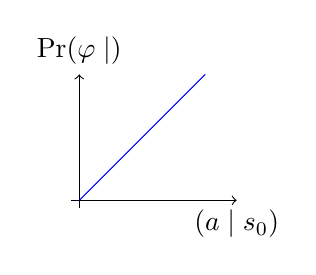
\begin{tikzpicture}[scale=2]
 \draw[->] (-0.05, 0) -- (1, 0) node[below]{$\sched(a \mid s_0 )$};
  	\draw[->] (0, -0.05) -- (0, 0.8) node[above] {$\Pr( \varphi \mid \sched)$};
  	%\draw[-,dashed] (0.4,0) -- (0.4,0.5184);
  	%\draw[-,dashed] (0.0,0.5184) -- (0.4,0.5184);
  \draw[ domain=0:0.8, smooth, variable=\x, blue] plot ({\x}, {\x});
\end{tikzpicture}
\caption{Probability to reach $\target$}
\label{fig:minimal:soft}
\end{subfigure}
\begin{subfigure}{0.36\columnwidth}
\centering
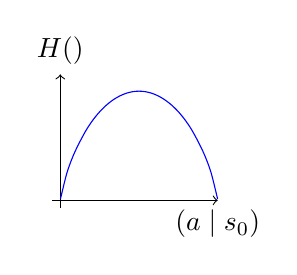
\begin{tikzpicture}[scale=2]	
 \draw[->] (-0.05, 0) -- (1, 0) node[below]{$\sched(a \mid s_0 )$};
  	\draw[->] (0, -0.05) -- (0, 0.8) node[above] {$H(\sched)$};
  	%\draw[-,dashed] (0.4,0) -- (0.4,0.5184);
  	%\draw[-,dashed] (0.0,0.5184) -- (0.4,0.5184);
  \draw[ domain=0.001:0.999, smooth, variable=\x, blue] plot ({\x}, {-\x * ln(\x) - (1 - \x)*  ln(1-\x)});
\end{tikzpicture}
\caption{Causal Entropy}
\label{fig:minimal:entropy}
\end{subfigure}

\caption{Minimal ERCI problem with $\varphi = ( \last{\xi} = \target )$}
\end{figure}


\subsection{Preprocessing}
To ease the technical exposition, without loss of generality, we make
the following assumptions\footnote{We argue that these assumptions are
indeed w.l.o.g.\ in Sec.~\ref{sec:assumptions}}: We assume the graph
structure underlying the SG is finite and acyclic -- and thus all paths
are finite length. When considering $\tau$-bounded path properties,
this assumption is naturally realized by a $\tau$-step unrolling the
SG's graph, i.e., augmenting the state space with a counter from $0$ to $\tau$.
One may then represent this unrolled graph as a binary
decision diagram, resulting in a (typically) concise graph that grows
proportional to the horizon and minimal\footnotemark state space augmentation
required~\cite{DBLP:conf/cav/Vazquez-Chanlatte20}.

\footnotetext{Formally, the state space is quotiented by distinguishablity under $\soft$ and $\hard$.}

Next, in order to ensure the hard constraint, $\hard$, we
calculate all states from which the $\pTwo$-player can enforce
violating the hard constraint. Such states are identifiable using a single
topologically ordered pass over $\sg$ from the leaves to the root.  We remove
such states along with their in- and outgoing transitions. Any
$\pOne$-policy now satisfies the hard constraint. 
The remaining sink states are all merged into two states $\target$ and
$\sink$, based on membership in $\soft$, i.e.,
\begin{equation}
  \begin{split}
    \last{\path} = \target ~\implies~ \path \in \soft\\
    \last{\path} = \sink ~\implies~ \path \notin \soft
  \end{split}.
\end{equation}

\noindent 
Together, we obtain the following (core) ERCI problem.
\begin{mdframed}
\textbf{The Core ERCI Problem}:
Given an finite acyclic SG $\sg$, with sink states, $\target$ and $\sink$, and thresholds $\scthreshold \in (0,1)$ and $\randomness \in [0,\infty)$,  find a $\pOne$-policy $\pOneSched$  such that for every $\pTwo$-policy $\pTwoSched$
\begin{enumerate}
\item (\emph{soft constraint)}
  $\Pr(\last{\xi} = \target \mid \sched) \geq \scthreshold$
\item (\emph{randomness constraint}) $H(\sigma) \geq \randomness$
\end{enumerate}
where  $\sched = \langle \pOneSched, \pTwoSched \rangle$.
\end{mdframed}

\begin{example}
	In Fig.~\ref{fig:minimal:mdp} we show a (deterministic) MDP and we plot for all schedulers the induced probability to reach $\target$ and the induced causal entropy, in Fig.~\ref{fig:minimal:soft} and \ref{fig:minimal:entropy}, respectively. 
	We see that taking action $a$ with increasing probability yields obviously to a larger probability to reach $\target$, whereas taking action $a$ and $b$ uniformly at random is optimal for the entropy. 
\end{example}



%%% Local Variables:
%%% mode: latex
%%% TeX-master: "main"
%%% End:
